% This file is generated by the MATLAB m-file laprint.m. It can be included
% into LaTeX documents using the packages graphicx, color and psfrag.
% It is accompanied by a postscript file. A sample LaTeX file is:
%    \documentclass{article}\usepackage{graphicx,color,psfrag}
%    \begin{document}% This file is generated by the MATLAB m-file laprint.m. It can be included
% into LaTeX documents using the packages graphicx, color and psfrag.
% It is accompanied by a postscript file. A sample LaTeX file is:
%    \documentclass{article}\usepackage{graphicx,color,psfrag}
%    \begin{document}% This file is generated by the MATLAB m-file laprint.m. It can be included
% into LaTeX documents using the packages graphicx, color and psfrag.
% It is accompanied by a postscript file. A sample LaTeX file is:
%    \documentclass{article}\usepackage{graphicx,color,psfrag}
%    \begin{document}% This file is generated by the MATLAB m-file laprint.m. It can be included
% into LaTeX documents using the packages graphicx, color and psfrag.
% It is accompanied by a postscript file. A sample LaTeX file is:
%    \documentclass{article}\usepackage{graphicx,color,psfrag}
%    \begin{document}\input{Response}\end{document}
% See http://www.mathworks.de/matlabcentral/fileexchange/loadFile.do?objectId=4638
% for recent versions of laprint.m.
%
% created by:           LaPrint version 3.16 (13.9.2004)
% created on:           09-May-2011 10:17:33
% eps bounding box:     15 cm x 11.25 cm
% comment:              
%
\begin{psfrags}%
\psfragscanon%
%
% text strings:
\psfrag{s05}[t][t]{\color[rgb]{0,0,0}\setlength{\tabcolsep}{0pt}\begin{tabular}{c}{\Large $f\tau$}\end{tabular}}%
\psfrag{s06}[b][b]{\color[rgb]{0,0,0}\setlength{\tabcolsep}{0pt}\begin{tabular}{c}{\Large $\left|\widetilde{w}(f)\right|$}\end{tabular}}%
\psfrag{s10}[][]{\color[rgb]{0,0,0}\setlength{\tabcolsep}{0pt}\begin{tabular}{c} \end{tabular}}%
\psfrag{s11}[][]{\color[rgb]{0,0,0}\setlength{\tabcolsep}{0pt}\begin{tabular}{c} \end{tabular}}%
\psfrag{s12}[l][l]{\color[rgb]{0,0,0}{\large $\widetilde{w}_\mathrm{PB}(f;\beta =14,\epsilon = 0.1)$}}%
\psfrag{s13}[l][l]{\color[rgb]{0,0,0}{\large $\widetilde{w}_\mathrm{R}(f)$}}%
\psfrag{s14}[l][l]{\color[rgb]{0,0,0}{\large $\widetilde{w}_\mathrm{BH}(f)$}}%
\psfrag{s15}[l][l]{\color[rgb]{0,0,0}{\large $\widetilde{w}_\mathrm{N}(f)$}}%
\psfrag{s16}[l][l]{\color[rgb]{0,0,0}{\large $\widetilde{w}_\mathrm{KB}(f;\beta = 14)$}}%
\psfrag{s17}[l][l]{\color[rgb]{0,0,0}{\large $\widetilde{w}_\mathrm{P}(f;\epsilon = 0.1)$}}%
\psfrag{s18}[l][l]{\color[rgb]{0,0,0}{\large $\widetilde{w}_\mathrm{PB}(f;\beta =14,\epsilon = 0.1)$}}%
%
% xticklabels:
\psfrag{x01}[t][t]{$10^{0}$}%
\psfrag{x02}[t][t]{$10^{1}$}%
\psfrag{x03}[t][t]{$10^{2}$}%
%
% yticklabels:
\psfrag{v01}[r][r]{$10^{-10}$}%
\psfrag{v02}[r][r]{$10^{-8}$}%
\psfrag{v03}[r][r]{$10^{-6}$}%
\psfrag{v04}[r][r]{$10^{-4}$}%
\psfrag{v05}[r][r]{$10^{-2}$}%
\psfrag{v06}[r][r]{$10^{0}$}%
%
% Figure:
\resizebox{12cm}{!}{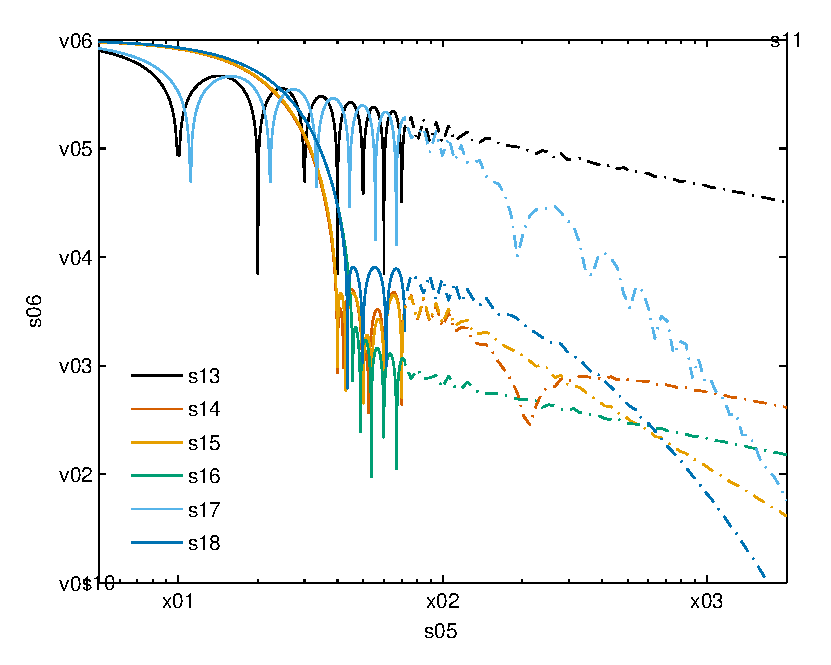
\includegraphics{Response.eps}}%
\end{psfrags}%
%
% End Response.tex
\end{document}
% See http://www.mathworks.de/matlabcentral/fileexchange/loadFile.do?objectId=4638
% for recent versions of laprint.m.
%
% created by:           LaPrint version 3.16 (13.9.2004)
% created on:           09-May-2011 10:17:33
% eps bounding box:     15 cm x 11.25 cm
% comment:              
%
\begin{psfrags}%
\psfragscanon%
%
% text strings:
\psfrag{s05}[t][t]{\color[rgb]{0,0,0}\setlength{\tabcolsep}{0pt}\begin{tabular}{c}{\Large $f\tau$}\end{tabular}}%
\psfrag{s06}[b][b]{\color[rgb]{0,0,0}\setlength{\tabcolsep}{0pt}\begin{tabular}{c}{\Large $\left|\widetilde{w}(f)\right|$}\end{tabular}}%
\psfrag{s10}[][]{\color[rgb]{0,0,0}\setlength{\tabcolsep}{0pt}\begin{tabular}{c} \end{tabular}}%
\psfrag{s11}[][]{\color[rgb]{0,0,0}\setlength{\tabcolsep}{0pt}\begin{tabular}{c} \end{tabular}}%
\psfrag{s12}[l][l]{\color[rgb]{0,0,0}{\large $\widetilde{w}_\mathrm{PB}(f;\beta =14,\epsilon = 0.1)$}}%
\psfrag{s13}[l][l]{\color[rgb]{0,0,0}{\large $\widetilde{w}_\mathrm{R}(f)$}}%
\psfrag{s14}[l][l]{\color[rgb]{0,0,0}{\large $\widetilde{w}_\mathrm{BH}(f)$}}%
\psfrag{s15}[l][l]{\color[rgb]{0,0,0}{\large $\widetilde{w}_\mathrm{N}(f)$}}%
\psfrag{s16}[l][l]{\color[rgb]{0,0,0}{\large $\widetilde{w}_\mathrm{KB}(f;\beta = 14)$}}%
\psfrag{s17}[l][l]{\color[rgb]{0,0,0}{\large $\widetilde{w}_\mathrm{P}(f;\epsilon = 0.1)$}}%
\psfrag{s18}[l][l]{\color[rgb]{0,0,0}{\large $\widetilde{w}_\mathrm{PB}(f;\beta =14,\epsilon = 0.1)$}}%
%
% xticklabels:
\psfrag{x01}[t][t]{$10^{0}$}%
\psfrag{x02}[t][t]{$10^{1}$}%
\psfrag{x03}[t][t]{$10^{2}$}%
%
% yticklabels:
\psfrag{v01}[r][r]{$10^{-10}$}%
\psfrag{v02}[r][r]{$10^{-8}$}%
\psfrag{v03}[r][r]{$10^{-6}$}%
\psfrag{v04}[r][r]{$10^{-4}$}%
\psfrag{v05}[r][r]{$10^{-2}$}%
\psfrag{v06}[r][r]{$10^{0}$}%
%
% Figure:
\resizebox{12cm}{!}{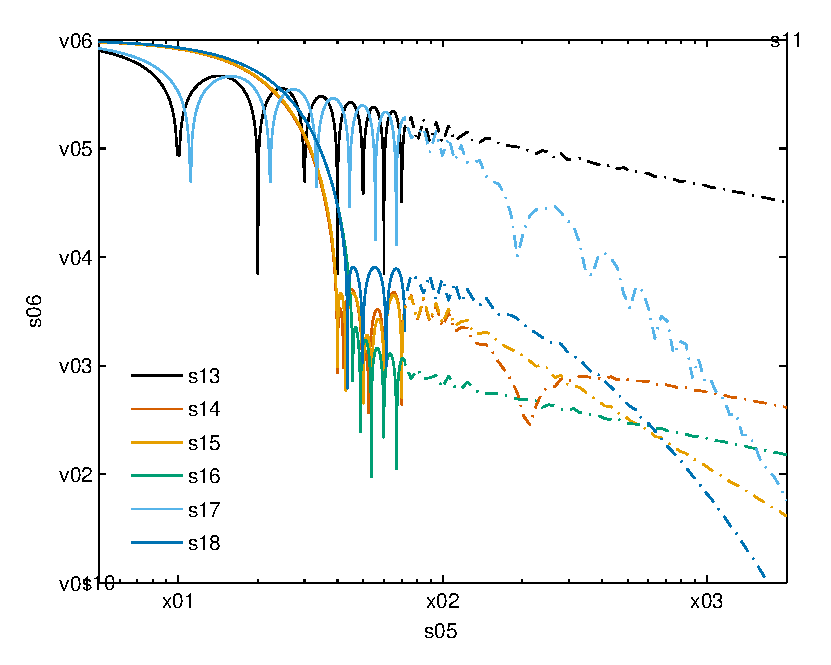
\includegraphics{Response.eps}}%
\end{psfrags}%
%
% End Response.tex
\end{document}
% See http://www.mathworks.de/matlabcentral/fileexchange/loadFile.do?objectId=4638
% for recent versions of laprint.m.
%
% created by:           LaPrint version 3.16 (13.9.2004)
% created on:           09-May-2011 10:17:33
% eps bounding box:     15 cm x 11.25 cm
% comment:              
%
\begin{psfrags}%
\psfragscanon%
%
% text strings:
\psfrag{s05}[t][t]{\color[rgb]{0,0,0}\setlength{\tabcolsep}{0pt}\begin{tabular}{c}{\Large $f\tau$}\end{tabular}}%
\psfrag{s06}[b][b]{\color[rgb]{0,0,0}\setlength{\tabcolsep}{0pt}\begin{tabular}{c}{\Large $\left|\widetilde{w}(f)\right|$}\end{tabular}}%
\psfrag{s10}[][]{\color[rgb]{0,0,0}\setlength{\tabcolsep}{0pt}\begin{tabular}{c} \end{tabular}}%
\psfrag{s11}[][]{\color[rgb]{0,0,0}\setlength{\tabcolsep}{0pt}\begin{tabular}{c} \end{tabular}}%
\psfrag{s12}[l][l]{\color[rgb]{0,0,0}{\large $\widetilde{w}_\mathrm{PB}(f;\beta =14,\epsilon = 0.1)$}}%
\psfrag{s13}[l][l]{\color[rgb]{0,0,0}{\large $\widetilde{w}_\mathrm{R}(f)$}}%
\psfrag{s14}[l][l]{\color[rgb]{0,0,0}{\large $\widetilde{w}_\mathrm{BH}(f)$}}%
\psfrag{s15}[l][l]{\color[rgb]{0,0,0}{\large $\widetilde{w}_\mathrm{N}(f)$}}%
\psfrag{s16}[l][l]{\color[rgb]{0,0,0}{\large $\widetilde{w}_\mathrm{KB}(f;\beta = 14)$}}%
\psfrag{s17}[l][l]{\color[rgb]{0,0,0}{\large $\widetilde{w}_\mathrm{P}(f;\epsilon = 0.1)$}}%
\psfrag{s18}[l][l]{\color[rgb]{0,0,0}{\large $\widetilde{w}_\mathrm{PB}(f;\beta =14,\epsilon = 0.1)$}}%
%
% xticklabels:
\psfrag{x01}[t][t]{$10^{0}$}%
\psfrag{x02}[t][t]{$10^{1}$}%
\psfrag{x03}[t][t]{$10^{2}$}%
%
% yticklabels:
\psfrag{v01}[r][r]{$10^{-10}$}%
\psfrag{v02}[r][r]{$10^{-8}$}%
\psfrag{v03}[r][r]{$10^{-6}$}%
\psfrag{v04}[r][r]{$10^{-4}$}%
\psfrag{v05}[r][r]{$10^{-2}$}%
\psfrag{v06}[r][r]{$10^{0}$}%
%
% Figure:
\resizebox{12cm}{!}{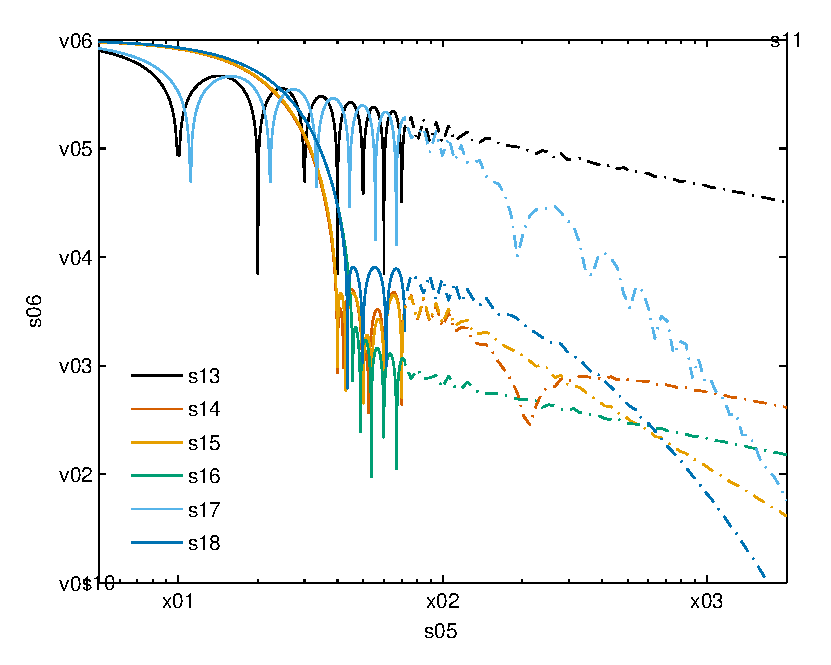
\includegraphics{Response.eps}}%
\end{psfrags}%
%
% End Response.tex
\end{document}
% See http://www.mathworks.de/matlabcentral/fileexchange/loadFile.do?objectId=4638
% for recent versions of laprint.m.
%
% created by:           LaPrint version 3.16 (13.9.2004)
% created on:           09-May-2011 10:17:33
% eps bounding box:     15 cm x 11.25 cm
% comment:              
%
\begin{psfrags}%
\psfragscanon%
%
% text strings:
\psfrag{s05}[t][t]{\color[rgb]{0,0,0}\setlength{\tabcolsep}{0pt}\begin{tabular}{c}{\Large $f\tau$}\end{tabular}}%
\psfrag{s06}[b][b]{\color[rgb]{0,0,0}\setlength{\tabcolsep}{0pt}\begin{tabular}{c}{\Large $\left|\widetilde{w}(f)\right|$}\end{tabular}}%
\psfrag{s10}[][]{\color[rgb]{0,0,0}\setlength{\tabcolsep}{0pt}\begin{tabular}{c} \end{tabular}}%
\psfrag{s11}[][]{\color[rgb]{0,0,0}\setlength{\tabcolsep}{0pt}\begin{tabular}{c} \end{tabular}}%
\psfrag{s12}[l][l]{\color[rgb]{0,0,0}{\large $\widetilde{w}_\mathrm{PB}(f;\beta =14,\epsilon = 0.1)$}}%
\psfrag{s13}[l][l]{\color[rgb]{0,0,0}{\large $\widetilde{w}_\mathrm{R}(f)$}}%
\psfrag{s14}[l][l]{\color[rgb]{0,0,0}{\large $\widetilde{w}_\mathrm{BH}(f)$}}%
\psfrag{s15}[l][l]{\color[rgb]{0,0,0}{\large $\widetilde{w}_\mathrm{N}(f)$}}%
\psfrag{s16}[l][l]{\color[rgb]{0,0,0}{\large $\widetilde{w}_\mathrm{KB}(f;\beta = 14)$}}%
\psfrag{s17}[l][l]{\color[rgb]{0,0,0}{\large $\widetilde{w}_\mathrm{P}(f;\epsilon = 0.1)$}}%
\psfrag{s18}[l][l]{\color[rgb]{0,0,0}{\large $\widetilde{w}_\mathrm{PB}(f;\beta =14,\epsilon = 0.1)$}}%
%
% xticklabels:
\psfrag{x01}[t][t]{$10^{0}$}%
\psfrag{x02}[t][t]{$10^{1}$}%
\psfrag{x03}[t][t]{$10^{2}$}%
%
% yticklabels:
\psfrag{v01}[r][r]{$10^{-10}$}%
\psfrag{v02}[r][r]{$10^{-8}$}%
\psfrag{v03}[r][r]{$10^{-6}$}%
\psfrag{v04}[r][r]{$10^{-4}$}%
\psfrag{v05}[r][r]{$10^{-2}$}%
\psfrag{v06}[r][r]{$10^{0}$}%
%
% Figure:
\resizebox{12cm}{!}{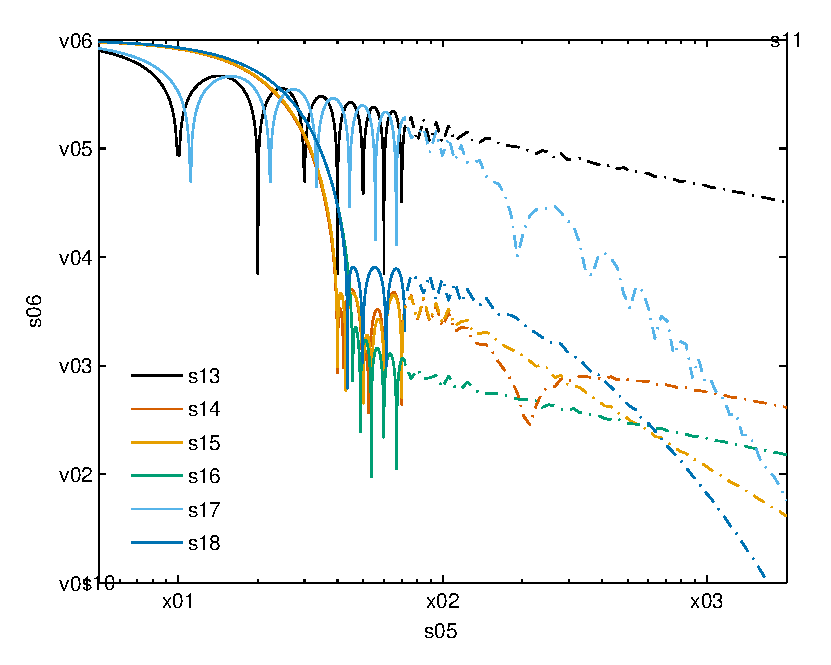
\includegraphics{Response.eps}}%
\end{psfrags}%
%
% End Response.tex
